\section{Methodology}
\label{sec:methodology}
In this section, the methodology proposed in this study is presented. Firstly, approach overview is described from a high-level perspective. Then, each stage in the methodology is presented together with their importance in the study, mathematical representations and definitions; and black-box diagrams. In the last section of this chapter, implementation details of this methodology in ProM framework is explained in detail with a software architecture overview.

\subsection{Approach Overview}
\label{subsec:approach-overview}
The approach proposed in this study consists of four main stages visualized in Figure~\ref{fig:approach-overview}. Firstly, in \textit{Process Model Mining}, process models are extracted from event logs for each organization with a user specified noise threshold. Secondly, in \textit{Performance Indicator Analysis}, event logs are replayed on process models and performance indicators are calculated for each organization then using these indicators, organizations are clustered based on how well they are operating. Thirdly, in \textit{Mismatch Pattern Analysis}, differences between process models of organizations are extracted with well-established mismatch patterns. Finally, in \textit{Recommendation Generation}, using the performance indicator clusterings and differences between process models, a set of recommendations for each organization is generated. In the following sections, each stage will be explained in detail with their mathematical backgrounds.

\begin{figure}
  \centering
  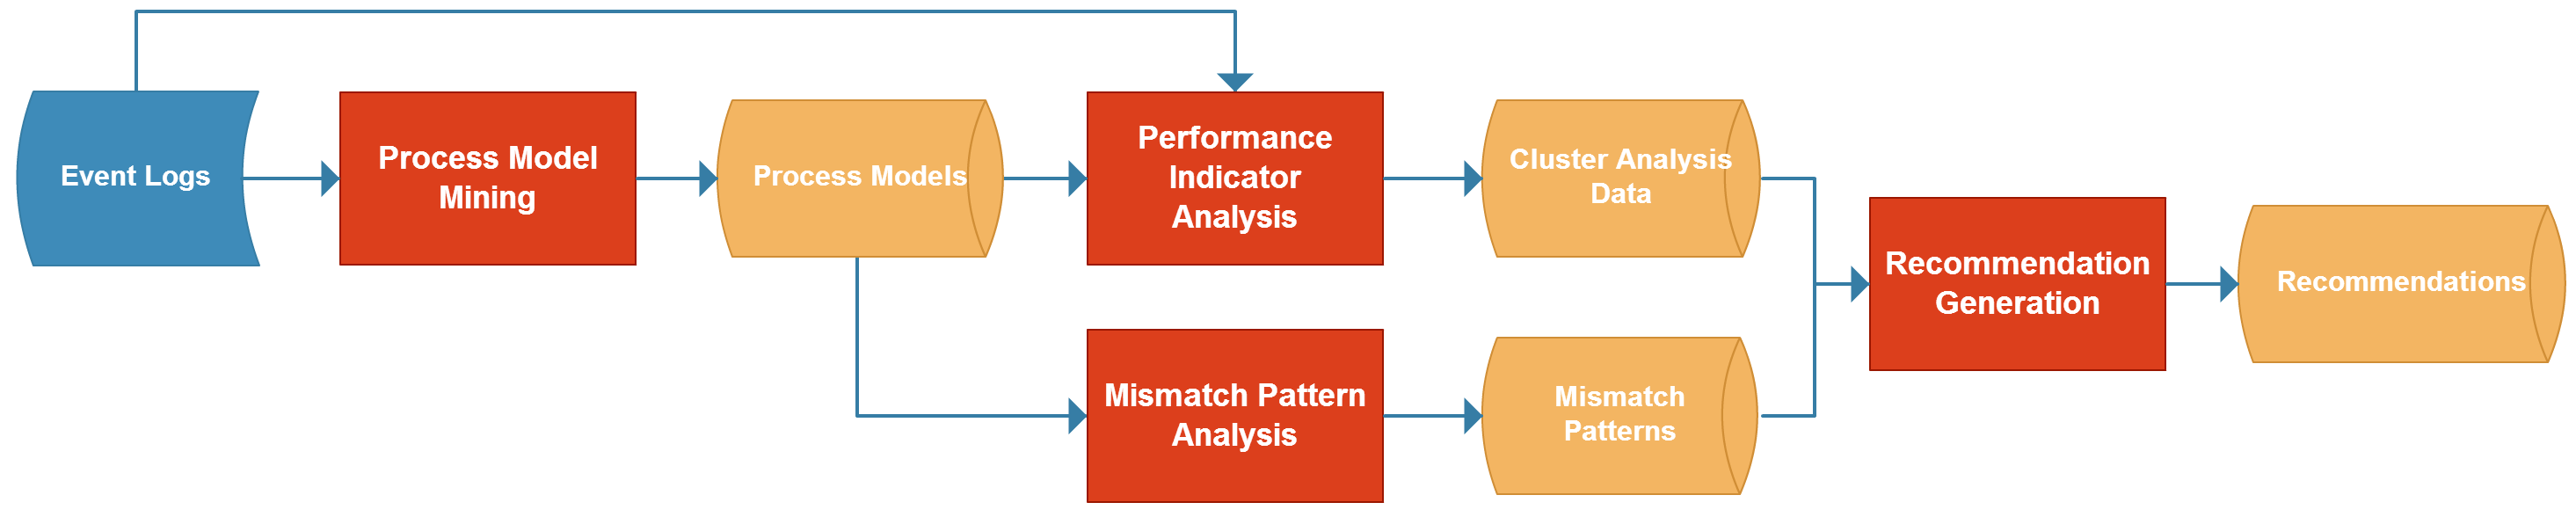
\includegraphics[width=\textwidth]{4_methodology/approach-overview}
  \caption{Overview of Methodology}
  \label{fig:approach-overview}
\end{figure}

\subsection{Process Model Mining}
\label{subsec:process-model-mining}
Process model mining in the proposed approach has the aim of creating reproducible and generalized process models from event logs. In order to achieve this aim, implementation of \textit{Inductive Miner Infrequent (IMi)}, which is proposed in \cite{leemans2014discoveringinfrequent} as an extension to \textit{Inductive Miner} to handle noise in the event logs, is used in this study. Considering the scope of this study, instead of computational details of \textit{Inductive Miner Infrequent (IMi)}; black-box representation is used to explain its usage in the methodology. In order to set a filtering threshold, a user-provided value between 0 to 1 is added as input to method in addition to event logs. As a result, workflow net is produced which is a sound and properly completed Petri net without deadlocks. Black-box of this stage is illustrated in Figure~\ref{fig:process-model-mining-blackbox} and this stage is called for every organization's event logs to create their own process models in Workflow net formalization.

\begin{figure}
  \centering
  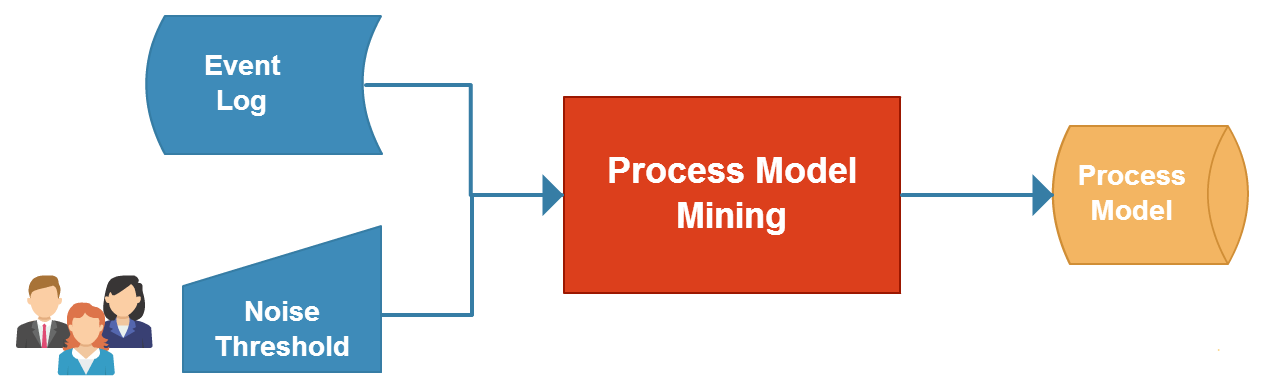
\includegraphics[width=0.5\textwidth]{4_methodology/process-model-mining-blackbox}
  \caption{Process Model Mining Stage as Black-box }
  \label{fig:process-model-mining-blackbox}
\end{figure}

\subsection{Performance Indicator Analysis}
\label{subsec:performance-indicator-analysis}
Performance indicator analysis stage focuses on calculating and analyzing the performance values using the event logs and mined process models. This stage consists of mainly two concepts as 
\begin{inparaenum}[\itshape a\upshape)]
\item alignment and calculation of performance indicators; and
\item clustering of organizations based on their performance values.
\end{inparaenum}
In order to evaluate the performance of an organization based on their process models and past activities; there is a number of indicators in time dimension, cost dimension and utilization \cite{van2011process}. However, in this study, process related performance values are considered since differences in the process models are studied in the next stages. With this reasoning, the following performance indicators are calculated and analyzed in this stage of methodology:
\begin{description}
	\item[Average Time Between Activities] For each activity in the process model, average time to reach other activity is calculated. This is a simple but powerful performance metric for organizations since it can yield the average time to complete one task based on a starting point. From the performance perspective, organizations want to minimize average time between activities to increase their throughput \cite{van2012replaying}.
	\item[Standard Deviation of Time Between Activities] Time between activities in real life is not stable and they deviate due to various reasons such as people responsible of tasks, size and the content of tasks or seasonality \cite{van2011process}. On the other hand, organizations want to be confident about their processes and therefore they want to minimize the deviation in the time between activities. Minimized deviation in time helps organizations to plan, act and re-organize the activities in the processes with high accuracy \cite{van2012replaying}. 
\end{description}

\subsubsection{Replay and Performance Indicator Calculation}
\label{subsubsec:replay-and-performance-summary}
Replay of event logs on process models is based on the idea of \textit{alignment} which is formalized in \cite{van2012replaying} and the basic assumption in this concept is that process models and event logs have the same activity labels. Alignment is based on \textit{moves in the model and log} and in order to have a successful replay where optimal alignment should be achieved. As proposed in \cite{adriansyah2011conformance,adriansyah2011towards}, $A^{*}$ algorithm which is a path-finding algorithm based on graphs is used to find optimal alignment of event logs on the process models. With the generated and user-specified inputs, replay and performance indicator calculation in the methodology can be visualized in Figure~\ref{fig:replay-and-performance-indicator-calculation}. For each organization, the steps in the diagram are followed with the corresponding event logs and process models; and the resulting process summaries are used for further analysis.

\begin{figure}
  \centering
  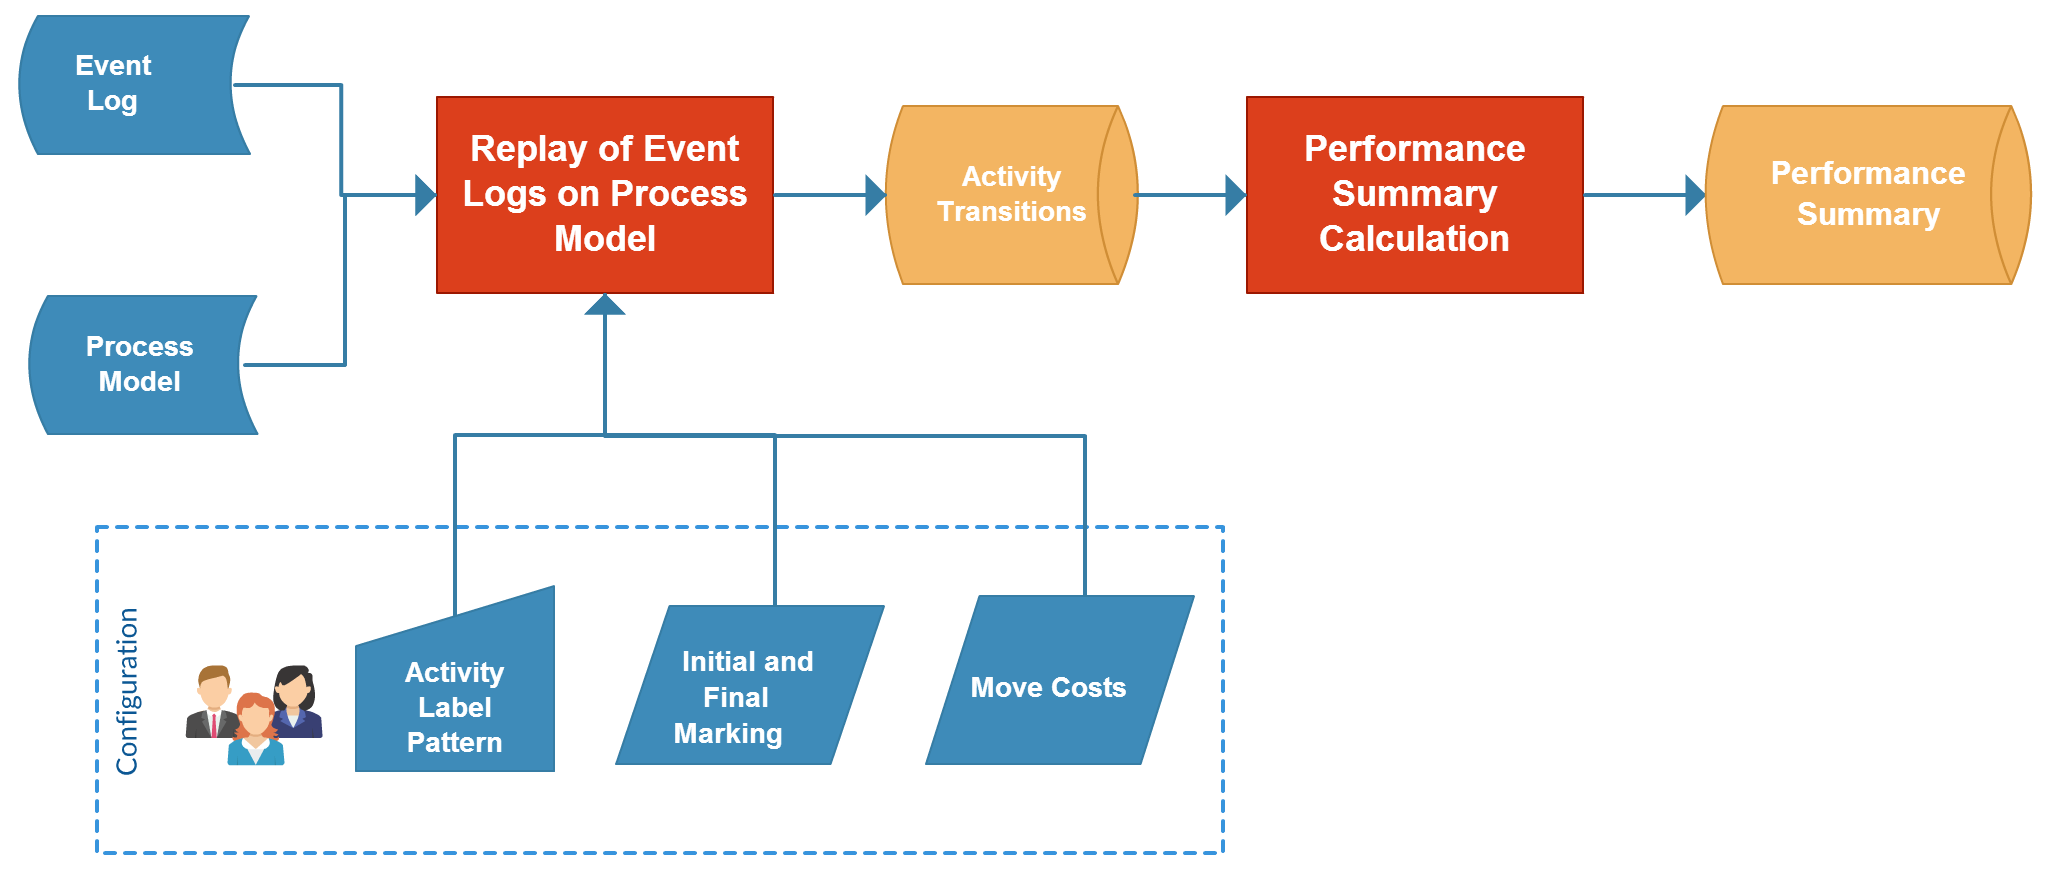
\includegraphics[width=\textwidth]{4_methodology/replay-and-performance-indicator-calculation}
  \caption{Replay and Performance Indicator Calculation Stage as Black-box}
  \label{fig:replay-and-performance-indicator-calculation}
\end{figure}

\subsubsection{Performance Indicator Clustering}
\label{subsubsec:performance-indicator-clustering}

Clustering is based on the idea of collecting the set of observations into clusters so that observations within the same cluster are similar whereas the observations from different clusters are dissimilar. In this thesis study, clustering is used to gather organizations based on their performance indicator data. In this study, a generic approach based on centroid-based clustering is exploited. For the fixed number of \textit{k} clusters, the approach is well-known as \textit{k-means clustering}. Considering the popularity of this approach and its extensions, random initialization based \textit{k-means++} approach from the study of Arthur and Vassilvitskii \cite{arthur2007} is used to cluster organizations. For each organization, \textit{Performance Summary} data is used as the data source in clustering. Since number of clusters are not known priori, k-means clustering is applied starting \textit{k} from 1 to the number of organizations. For each clustering with different number of clusters, SSE values are plotted and user is made to select the appropriate cluster size. For the selected cluster size, clustering related information is used to generate recommendations in the further steps. This stage of methodology can be visualized as an input-output system in Figure~\ref{fig:performance-indicator-clustering-blackbox}. 
\begin{figure}
  \centering
  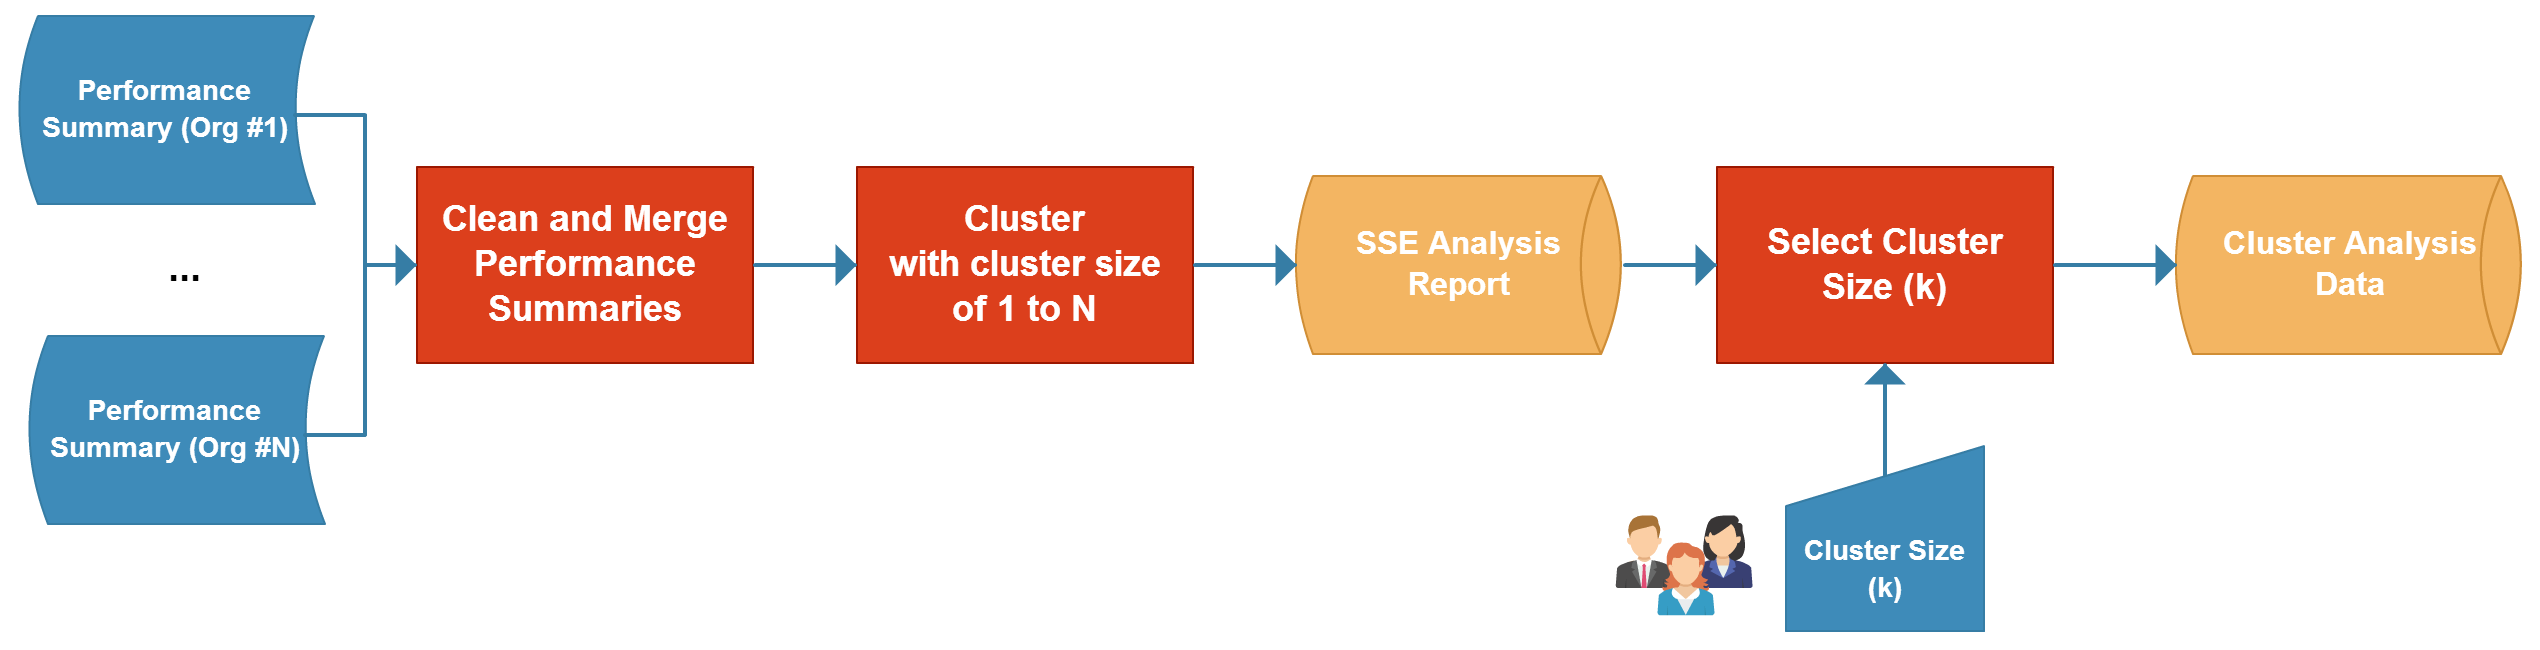
\includegraphics[width=\textwidth]{4_methodology/performance-indicator-clustering-blackbox}
  \caption{Performance Indicator Clustering Stage as Black-box }
  \label{fig:performance-indicator-clustering-blackbox}
\end{figure}




\subsection{Mismatch Pattern Analysis}
\label{subsec:mismatch-pattern-analysis}
In order to learn from other organizations, it is necessary to spot the differences between process models of different organizations. In this phase of methodology, differences between process models will be revealed by the mismatch patterns which are defined by Dijkman \cite{dijkman2007mismatch}. In the process mining stage, process models are mined to create Workflow nets; however, mismatch pattern definitions are closer to business environment and it is more suitable spot patterns in BPMN notation. Thus, mined process models are converted to BPMN models and then mismatch pattern analysis is applied. After spotting differences, mismatch patterns for activities and control flows are revealed for the organizations.

Business Process Modeling Notation (BPMN) is one of the widely accepted modeling language in the industry and its a standardized notation by the Object Management Group (OMG) since 2004. In this stage, BPMN formulation is used since mismatch patterns have roots in real-life business environment \cite{dijkman2007mismatch}. 

For each organization, mined process models are converted to BPMN models and mismatch patterns analysis is undertaken on them, in order to locate differences between two process models or cluster of process models. In addition, since performance indicators are calculated based on a starting and ending points in the process model, same approach is applied to locate mismatch patterns. In other words, differences of process models are located through a starting activity to an ending activity. When the complete set of mismatches between process models are required, this approach is used with starting and ending points as source and sink activities. For each organization, mismatch patterns are gathered and stored for the further analysis as visualized in Figure~\ref{fig:mismatch-pattern-analysis-blackbox}.

\begin{figure}
  \centering
  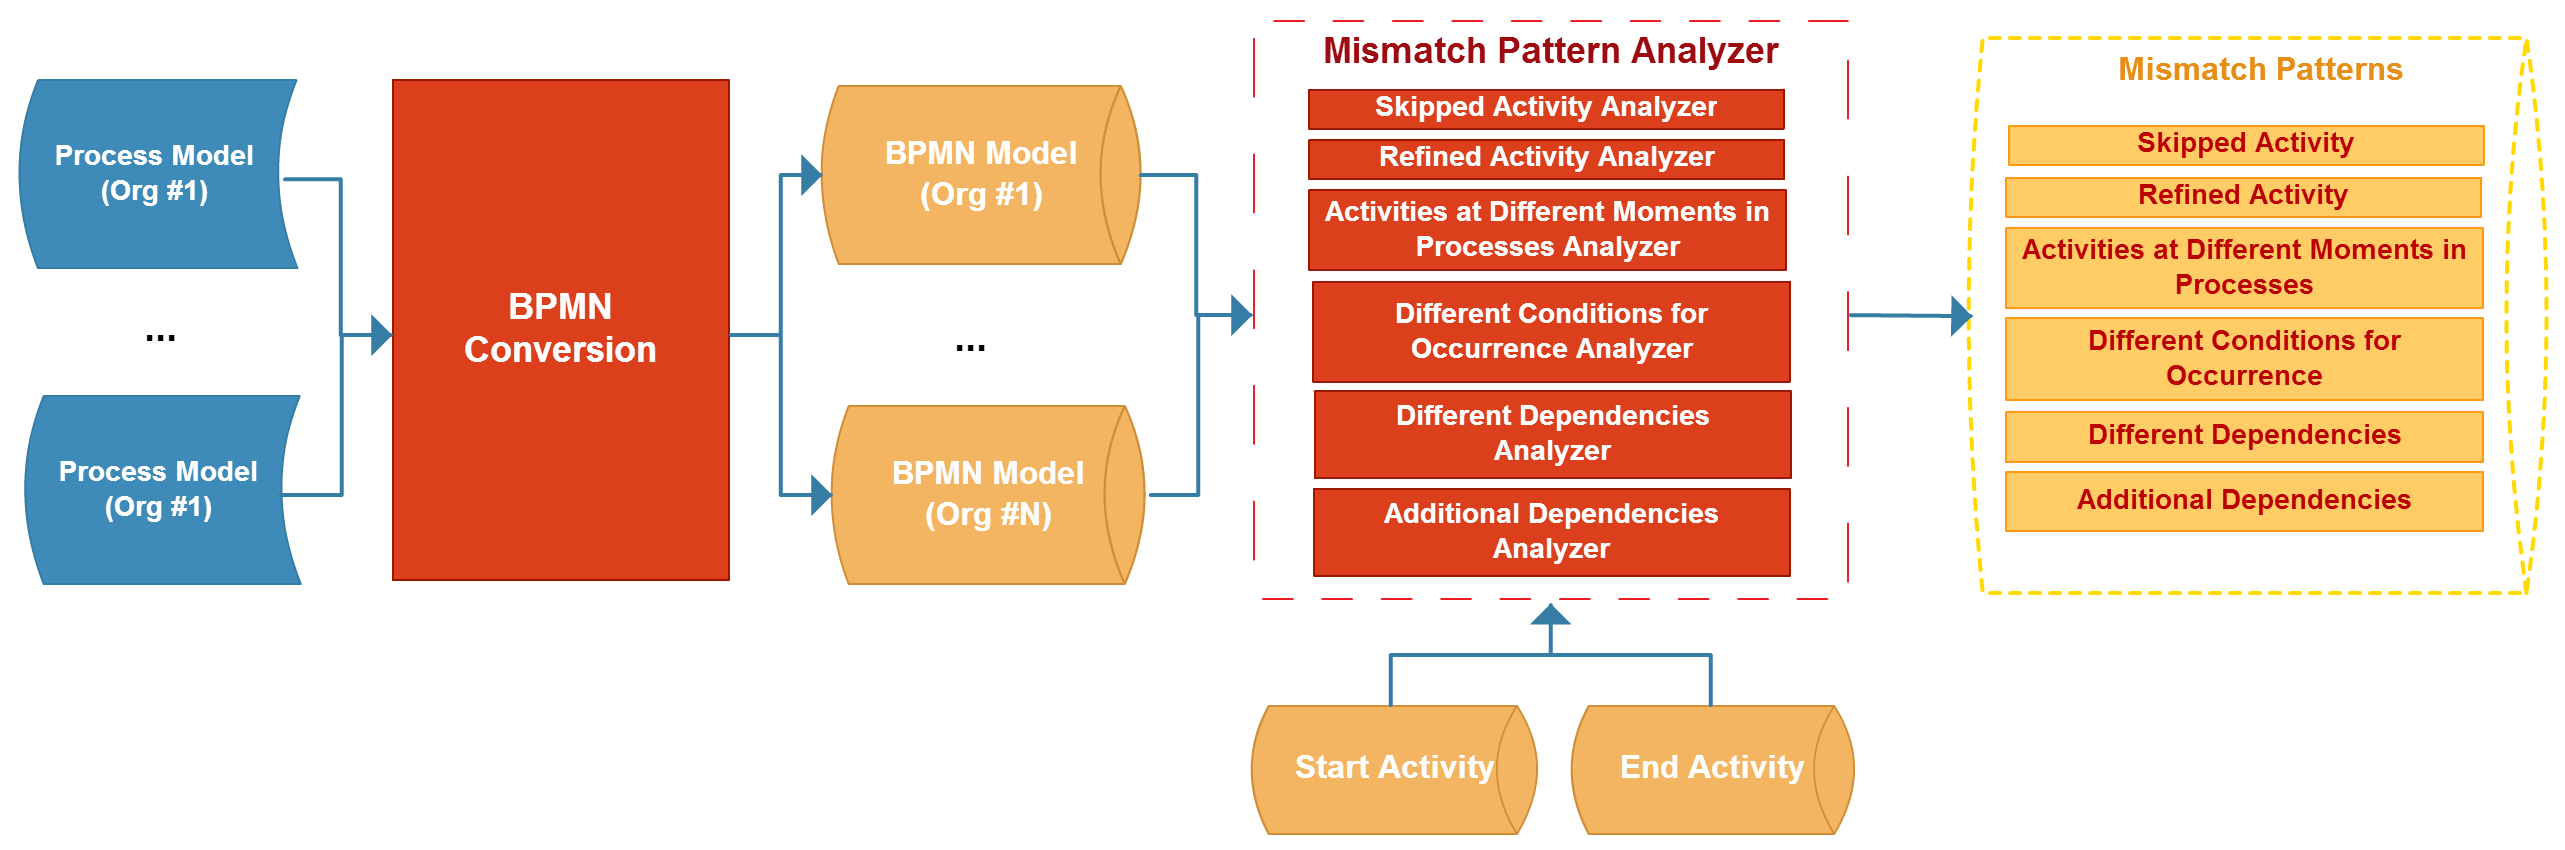
\includegraphics[width=\textwidth]{4_methodology/mismatch-pattern-analysis-blackbox}
  \caption{Mismatch Pattern Analysis Stage as Black-box}
  \label{fig:mismatch-pattern-analysis-blackbox}
\end{figure}

\subsection{Recommendation Generation}
\label{subsec:recommendation-generation}
Recommendation generation stage in the methodology is the final and core stage where all information retrieved from event logs until now are utilized. In this study, idea of recommendation is based on providing a set of mismatch patterns for each organization so that they can enhance their processes. These mismatch patterns are generated by comparing the process models of other organizations, particularly which are performing better in terms of their performance indicator values. In addition, clustering of organizations is undertaken to generalize the way of identifying which organizations perform better in this environment.

Algorithm of recommendation generation function is based on the idea of checking other clusters for a significant change in performance indicators, where significance is defined by the threshold provided by user. After finding significant difference, all organizations in other clusters are checked against mismatch patterns with the starting and ending activities defined in performance indicators. With this constraining, only mismatches which are located between the activities that causes high level of difference in performance indicators are analyzed. 

This stage of methodology can be visualized as gathering inputs of mismatch patterns data and cluster analysis data in Figure~\ref{fig:recommendation-generation-blackox}. In addition, a performance difference threshold is gathered from the user to specify how much difference between clusters is necessary to check for mismatch patterns and generate recommendations. This stage generates recommendation data for each organization which contains a set of mismatch patterns.
\begin{figure}
  \centering
  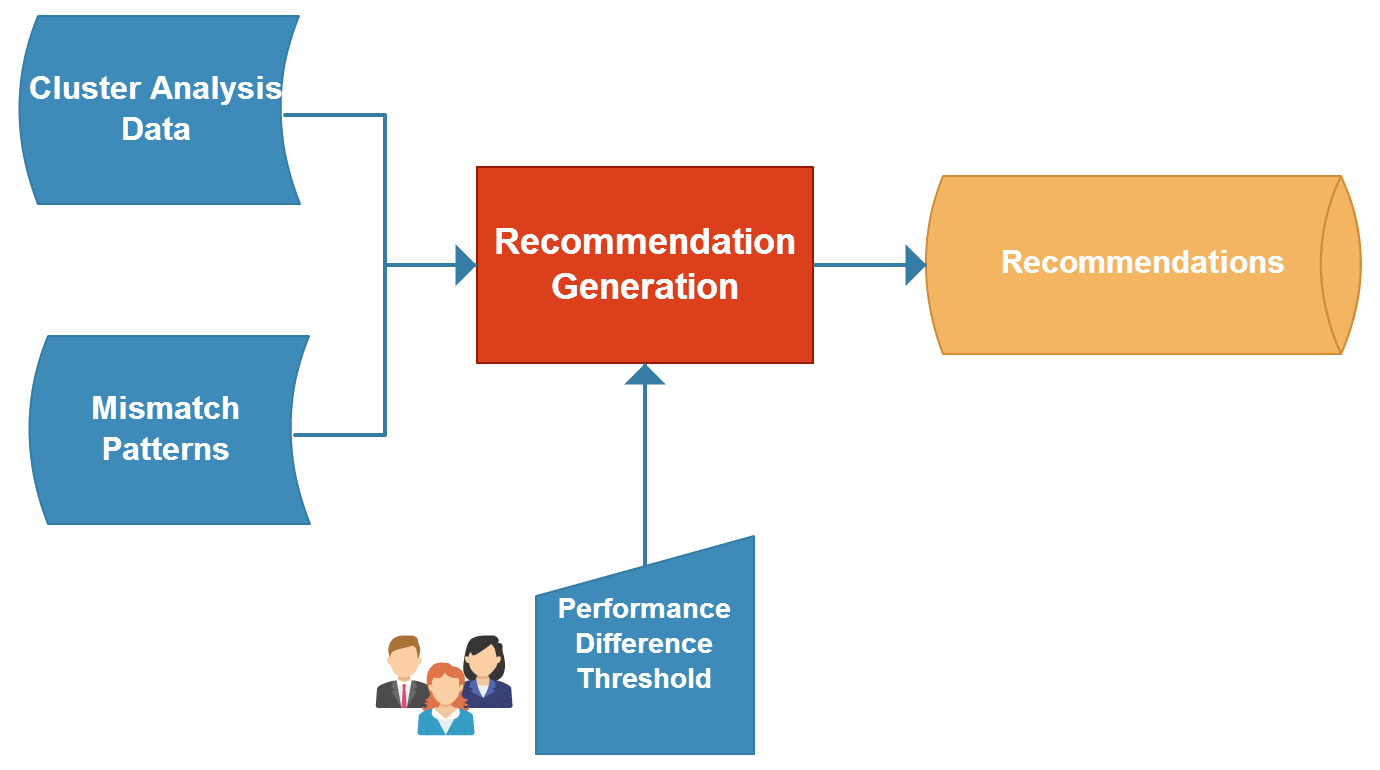
\includegraphics[width=0.7\textwidth]{4_methodology/recommendation-generation-blackbox}
  \caption{Recommendation Generation Stage as Black-box}
  \label{fig:recommendation-generation-blackox}
\end{figure}

\subsection{Implementation in ProM Framework}
\label{subsec:implementation}
Methodology of this thesis study is implemented in ProM \cite{verbeek2010prom}, which is an extensible framework that supports a wide variety of process mining techniques in form of plugins. ProM is an open source framework for process mining algorithms which provides a platform to users and developers. Aim of this framework is to create a standard process mining platform that is accepted in industry and academia with an active community. Approach of this thesis study is implemented with its each stage as a standalone plugin that enables extensions for further studies. Developed set of plugins are packaged with the name of \textit{CrossOrgProcMin}\footnote{\url{http://www.promtools.org/prom6/packages/CrossOrgProcMin}} and published open-source\footnote{\url{http://github.com/onuryilmaz/cross-org-proc-min}} being available in the latest version of ProM release. 

Approach of this study is divided into stand-alone stages where inputs and outputs between them are defined strictly. With the help of this understanding, each stage is developed as a stand-alone plug-in in ProM framework which can be called separately. For this aim, five plug-ins are developed to provide a high-level perspective. In addition, a set of utilities are developed to visualize and persistence of data in ProM environment. 